%! Author = wolfram_e_laube
%! Date = 06.05.24

\item[(b)]
\subsection{Task (b): Spectrum of $x[n]$}

\subsubsection{Problem Statement}
Analyze and visualize the spectrum of the discrete-time signal $x[n]$, obtained by sampling the continuous-time signal $x(t)$ at a frequency $f_s$, and elucidate the effects of sampling including aliasing.

\subsubsection{Mathematical Formulation}
\begin{itemize}
    \item \textbf{Sampling Frequency $f_s = 8$ kHz}
    \item \textbf{Baseband:} $[-f_s/2, f_s/2]$ or $[-4 \text{ kHz}, 4 \text{ kHz}]$
\end{itemize}

The spectrum $X(f)$ repeats every $f_s$, illustrating the aliasing effects:
\[
\text{Extended Frequency Range for Visualization: } [-3f_s, 3f_s]
\]
\[
\text{Repeated Spectrum: } \text{tile}( |X(f)|, 3)
\]

\subsubsection{Discussion}
The plot of $x[n]$ shows how the spectrum repeats every $f_s$ and highlights the baseband where the original spectrum lies within the Nyquist range. This visualization demonstrates the aliasing effect, where parts of the spectrum outside the baseband overlap with those inside it.

\begin{figure}[h]
    \centering
    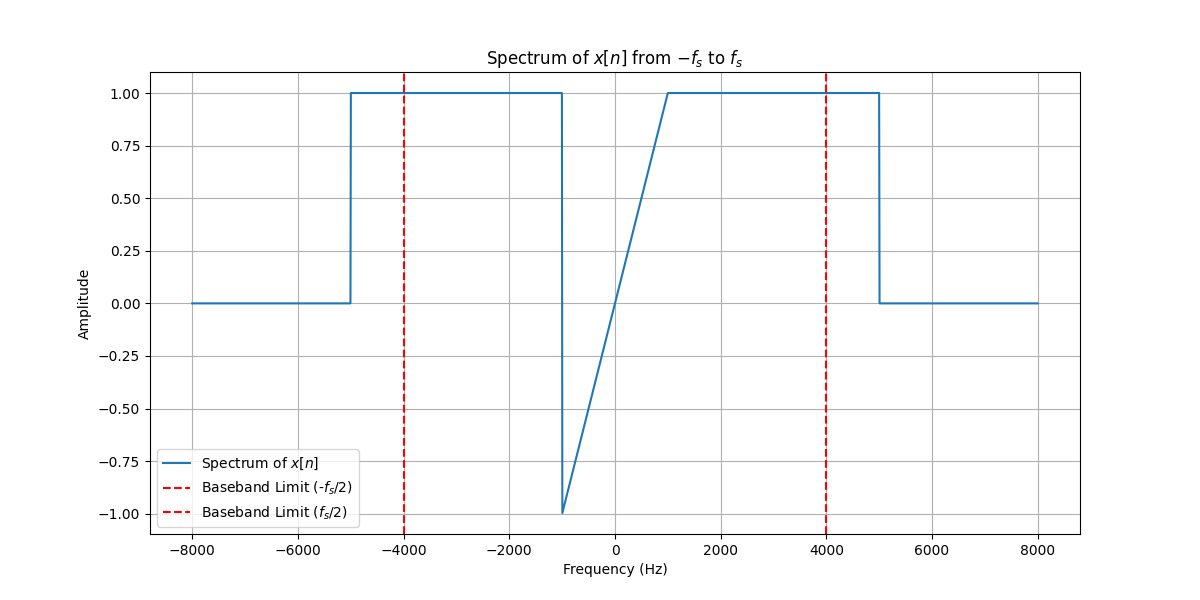
\includegraphics[width=0.49\textwidth]{fig/ex2_b_plot}
    \caption{Spectrum of \(x(t)\)}
    \label{fig:ex2_b_plot}
\end{figure}
